Rewrite the following subsections and try to keep the
writing of the thesis.

\subsection{Green Functions}
In this subsection, we discuss informally how to turn ODEs into integral equations mainly
by example. Our main tool for this are green functions.
Prior to discussing green functions, we offer several
examples.

\begin{notation}[$H$]
    We denote the Heaviside step function with:
    \begin{equation}
        H(x) = \begin{cases}
            0 & \text{ if } x<0 \\
            1 & \text{ else }
        \end{cases}.
    \end{equation}
\end{notation}

\begin{example}[$y'=y$ average condition]
    We will solve the equation:

    \begin{equation} \label{ydy int}
        y' = y,
    \end{equation}

    but this time with a different condition:

    \begin{equation}
        \int_{0}^{1} y(s) ds = e-1.
    \end{equation}

    The solution to this equation remains the same: $y(t) = e^{t}$.
    We define the corresponding source green function $G(t,x)$ for $y'$
    and this type of condition as follows:

    \begin{equation}
        G' = \delta(x-t), \quad \int_{0}^{1} G(s,x) ds = 0.
    \end{equation}

    Solving this equation yields:

    \begin{equation}
        G(t,x) = H(t-x) + x - 1.
    \end{equation}

    It is worth noting that we could have chosen a different
    green function corresponding to a different linear
    differential operator.

    At this point, it may not be clear, but using this green function,
    we can form the following integral equation for (\ref{ydy int}):

    \begin{equation} \label{int ydy int}
        y(t) = e - 1 + \int_{0}^{1} G(t,s) y(s) ds.
    \end{equation}

    Converting equation (\ref{int ydy int}) into a RRVE
    using RMC, we obtain:

    \begin{equation}\label{RRVE ydy int}
        Y(t) = e - 1 + 2B\left(\frac{1}{2}\right)Y(S)(H(t-S)+S-1),
    \end{equation}

    where $S \sim U$. We will skip the Python implementation
    of equation (\ref{RRVE ydy int}) as it does not provide any
    new information. Instead, we will plot realizations of
    equation (\ref{RRVE ydy int}) in Figure \ref{fig:ydy int}.

    \begin{figure}[h!]
        \centering
        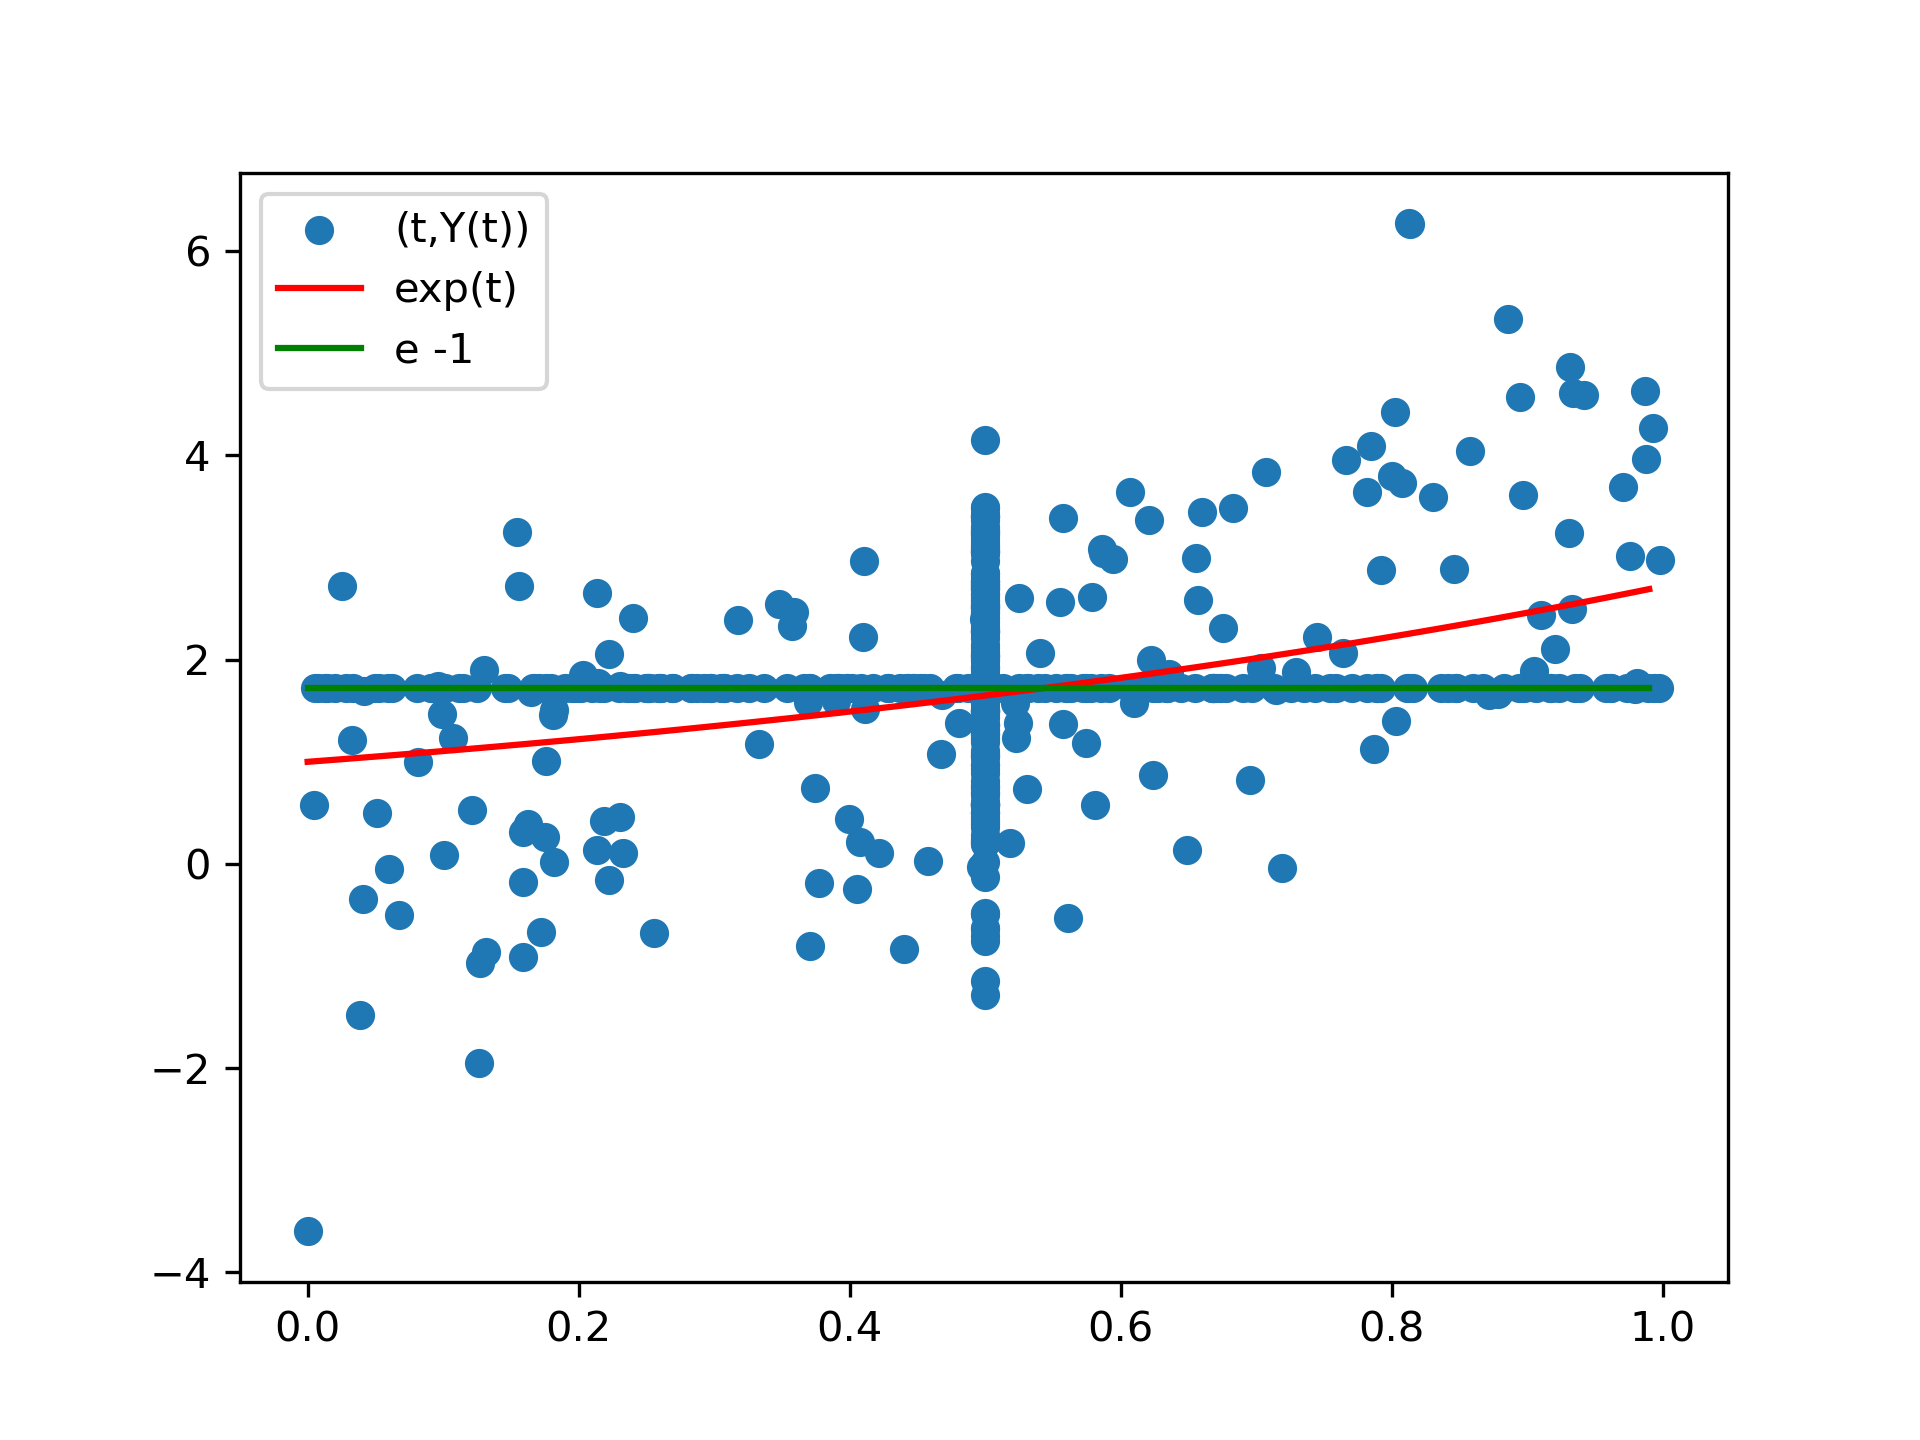
\includegraphics[width=0.8\textwidth]{plots/ydy int.png}
        \caption{Recursive calls of (\ref{RRVE ydy int}) when
            calling $Y(0.5)$ $300$ times. Points accumulate on
            the green line due to the Russian roulette,
            and at  $t=0.5$ because it is the starting
            value of the simulation.
        }
        \label{fig:ydy int}
    \end{figure}

\end{example}

% Green's function vs green function (check chatgpt for the answer)
\begin{definition}[green function]
    Vaguely speaking, we define the green function as a type
    of kernel function used to solve linear problems with linear
    conditions. The green function is the kernel that we
    place in front of the linear conditions or the source term,
    which we integrate over to obtain the solution. The green
    function possesses the property of satisfying either null
    linear conditions and a Dirac delta source term, or vice versa.
\end{definition}

\begin{related}[green function]
    Our notion of green function is similar to that in \cite{hwang_simulationtabulation_2001}.
\end{related}

\subsection{Fredholm Integral Equations}

\textcolor{green}{
    TODO:
    \begin{itemize}
        \item explain better the graph for coupled splitting
        \item add better explaination to coupled splitting
    \end{itemize}
}

The integral equations obtained in the previous subsection are Fredholm integral
equations of the second kind. In this subsection, we introduce a technique called
coupled splitting.


\begin{definition}[Fredholm equation of the second kind]
    A Fredholm equation of the second kind for $\varphi$  is of the following form:
    \begin{equation}
        \varphi(t)=f(t)+\lambda \int_a^b K(t, s) \varphi(s) ds.
    \end{equation}
    Given the kernel  $K(t, s)$  and  $ f(t)$.
\end{definition}

If both $K$ and $f$ satisfy certain regularity conditions, then for sufficiently
small $\lambda$, it is relatively straightforward to establish the existence
and uniqueness of solutions using a fixed-point argument.

\begin{example}[Dirichlet $y''=y$] \label{main dirichlet}
    The following ODE will be the main testing example for
    boundary value problems:
    \begin{equation} \label{eq:main dirichlet}
        y''=y, \quad y(b_{0}),y(b_{1}).
    \end{equation}
    The green functions corresponding to $y''$ and Dirichlet conditions are:

    \begin{align}
        P(t,x) & = \begin{cases}
                       \frac{b_{1}-t}{b_{1}-b_{0}} & \text{if } x = b_{0} \\
                       \frac{t-b_{0}}{b_{1}-b_{0}} & \text{if } x = b_{1}
                   \end{cases},       \\
        G(t,s) & = \begin{cases}
                       -\frac{(b_{1}-t)(s-b_{0})}{b_{1}-b_{0}} & \text{if } s<t \\
                       -\frac{(b_{1}-s)(t-b_{0})}{b_{1}-b_{0}} & \text{if } t<s
                   \end{cases}.
    \end{align}
    Straight from these green functions you get the following integral equation and RRVE:
    \begin{align} \label{inteq:main dirichlet}
        y(t) & = P(t,b_{0}) y(b_{0}) + P(t,b_{1}) y(b_{1}) +
        \int_{b_{0}}^{b_{1}} G(t,s)y(s) ds,                  \\
        Y(t) & = P(t,b_{0}) y(b_{0}) + P(t,b_{1}) y(b_{1})
        + l B\left(\frac{1}{l} \right)(b_{1}-b_{0}) G(t,S)y(S) , \label{RRVE:main dirichlet}
    \end{align}
    where $l \in \mathbb{R}$ the Russian roulette rate is and
    $S \sim \text{Uniform}(b_{1},b_{0})$.

\end{example}


\begin{example}[coupled splitting on (\ref{main dirichlet})] \label{ex:coupled splitting}
    In addition to normal splitting (see Definition \ref{def:splitting}),
    we can also split the domain in Equation (\ref{inteq:main dirichlet})
    as follows:

    \begin{align}\label{inteq:coupled splitting}
        y(t) & = P(t,b_{0}) y(b_{0}) + P(t,b_{1}) y(b_{1}) +
        \frac{1}{2} \int_{b_{0}}^{b_{1}} G(t,s)y(s) ds +
        \frac{1}{2} \int_{b_{0}}^{b_{1}} G(t,s)y(s) ds,                                             \\
        y(t) & = P(t,b_{0}) y(b_{0}) + P(t,b_{1}) y(b_{1}) + \label{inteq:coupled domain splitting}
        \int_{b_{0}}^{\frac{b_{1}+b_{0}}{2}} G(t,s)y(s) ds +
        \int_{\frac{b_{1}+b_{0}}{2}}^{b_{1}} G(t,s)y(s) ds.
    \end{align}

    By coupling, we can eliminate the additive branching recursion
    in the RRVEs corresponding to Equations (\ref{inteq:coupled splitting})
    and (\ref{inteq:coupled domain splitting}).
    This results in the following RRVE:

    \begin{equation} \label{RRVE:coupled splitting}
        X(t_{1},t_{2})=
        \begin{bmatrix}
            P(t_{1},b_{0}) & P(t_{1},b_{1}) \\
            P(t_{2},b_{0}) & P(t_{2},b_{1})
        \end{bmatrix}
        \begin{bmatrix}
            y(b_{0}) \\
            y(b_{1})
        \end{bmatrix}
        +
        W
        \begin{bmatrix}
            G(t_{1},S_{1}) & G(t_{1},S_{2}) \\
            G(t_{2},S_{1}) & G(t_{2},S_{2})
        \end{bmatrix}
        X(S_{1},S_{2}),
    \end{equation}
    where $W$ the right weighting matrix is
    (see code (\ref{py:coupled splitting})),
    and $S_{1}$ and $S_{2}$ can be chosen
    in various ways.
\end{example}

\begin{pythonn}[implementation of (\ref{RRVE:coupled splitting})] \label{py:coupled splitting}
    We implemented equation (\ref{RRVE:coupled splitting}) in example
    (\ref{ex:coupled splitting}) with recursion but in this case, it
    is also possible to implement it forwardly. \\
    \pythoncode{python code/coupled_splitting.py}

    % can probably make a better plot then this one
    \begin{figure}[h!]
        \centering
        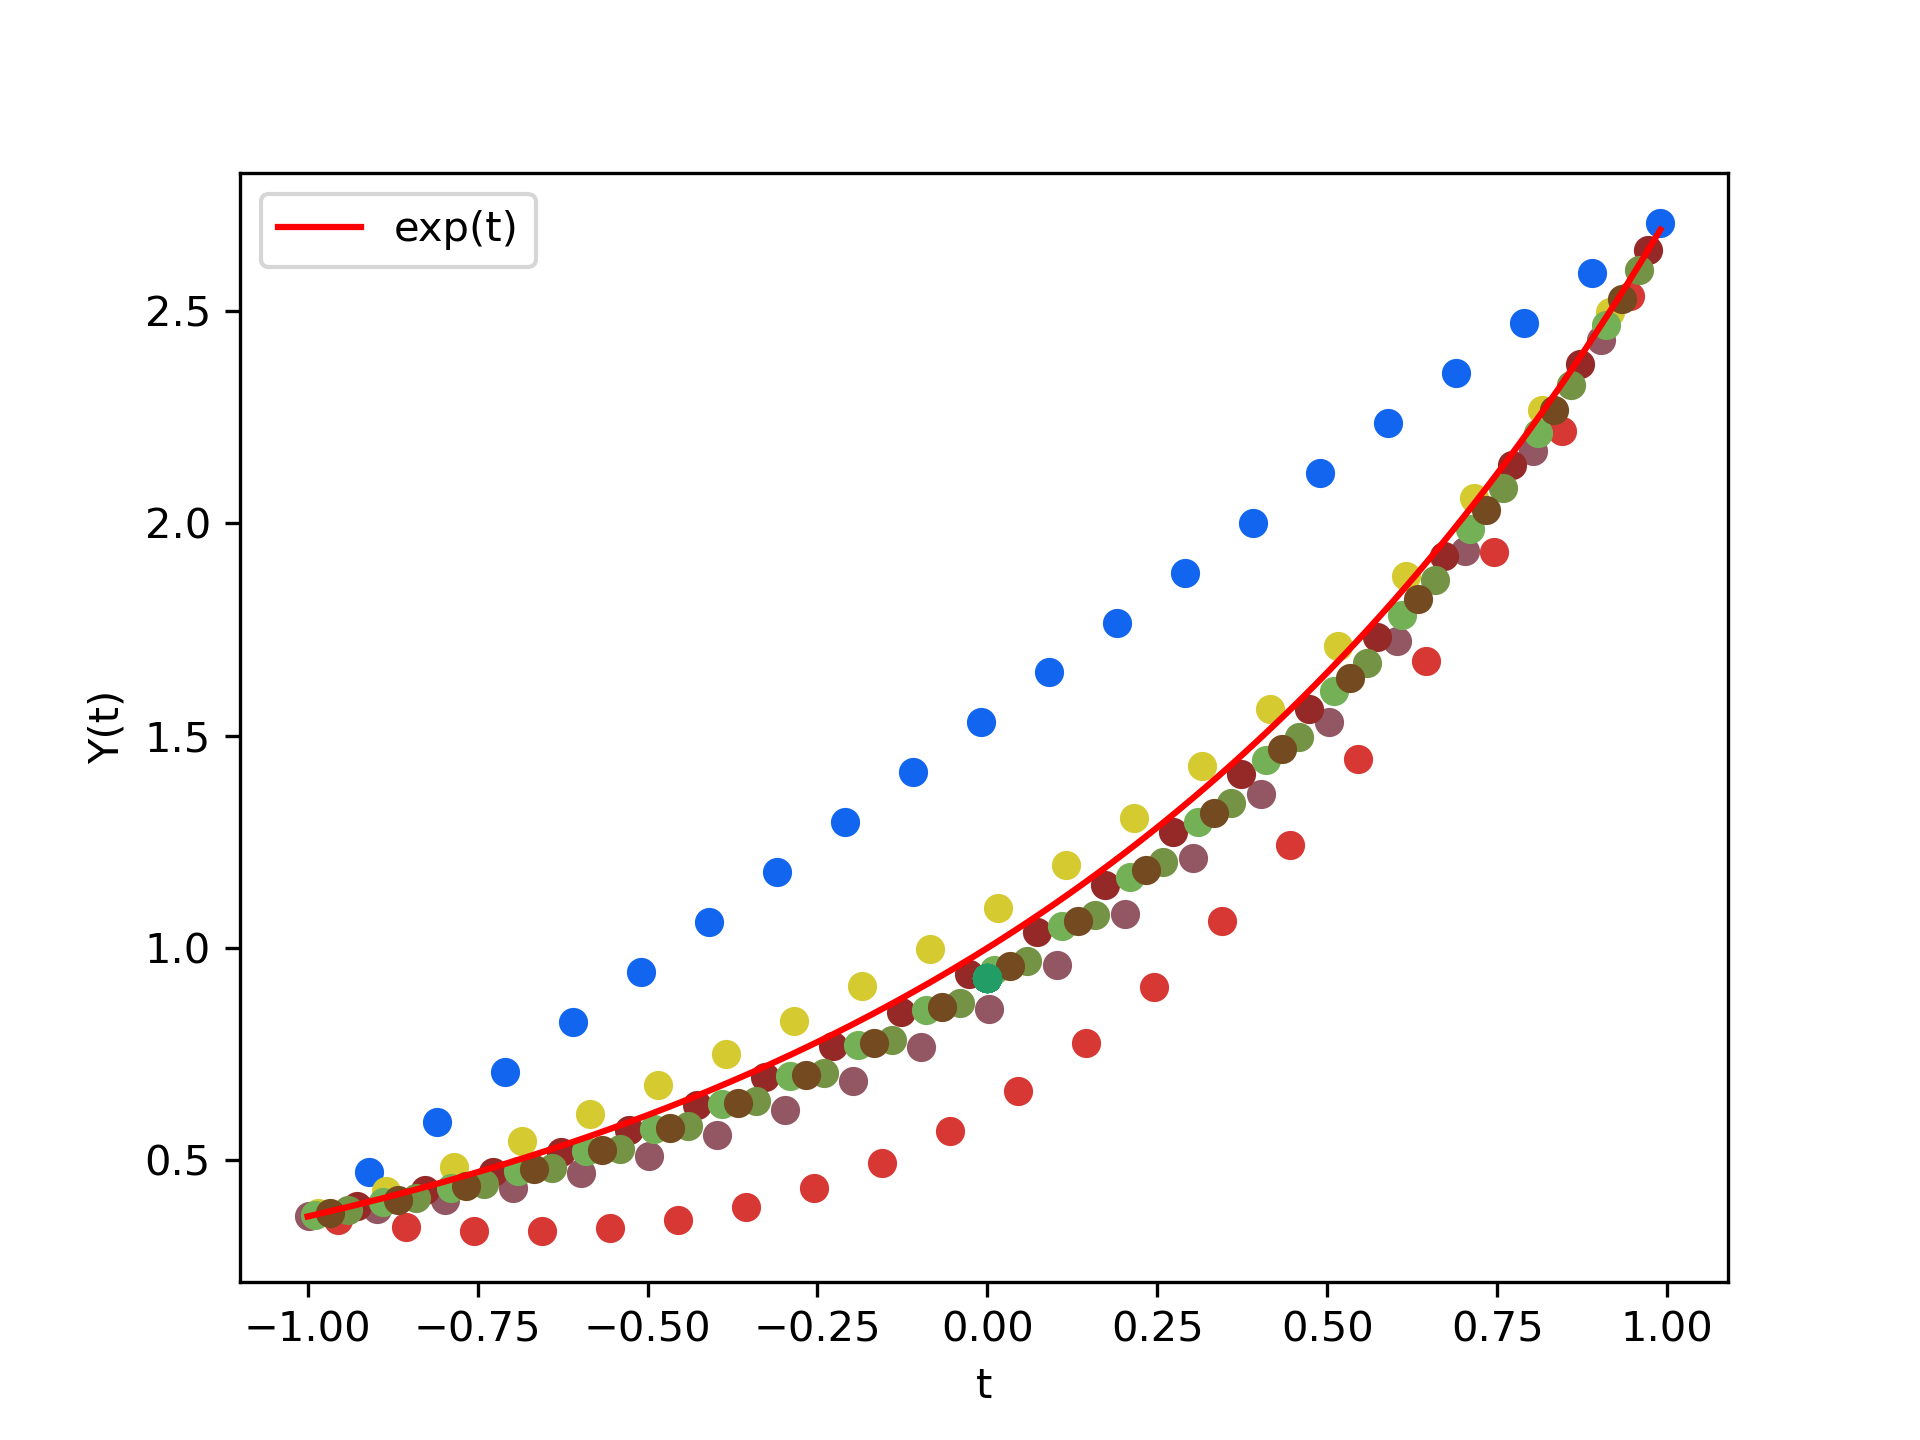
\includegraphics[width=0.8\textwidth]{plots/coupled split.png}
        \caption{Recursive calls of equation (\ref{RRVE:coupled splitting}) when
        calling $X(0)$ once,
        with a split size of $20$, $S_{j}$ are coupled such
        they are equally spaced and the coupling is colored.
        The initial conditions for this call are $y(-1)=e^{-1}$ and $y(1)=e^{1}$,
        with Russian roulette rate $l=1.2$.  }
        \label{fig:coupled splitting}
    \end{figure}
\end{pythonn}


Example (\ref{ex:coupled splitting}) does not
exploit the locality and smoothness of the problem.
We conjecture that coupled splitting can be particularly valuable when
dealing with linear Fredholm equations of the second kind,
especially in scenarios where MC integration surpasses
traditional integration methods. This holds true for
high-dimensional problems, non-smooth kernels, and
challenging domains. We conjecture that employing
coupled splitting in such cases can yield favorable results.

\begin{related}[coupled splitting]
    Coupled splitting is partly inspired by how \cite{sabelfeld_sparsified_2009}
    reduces variance by using bigger submatrices.
    Reusing samples for walk on sphere gets discussed
    in \cite{miller_boundary_2023} and \cite{bakbouk_mean_2023}.
\end{related}

Figure \ref{fig:coupled splitting}
resembles fixed-point iterations, leading us to hypothesize
that coupled splitting can achieve convergence in most cases
where a fixed-point argument holds true and the convergence
speed is very similar to fix-points methods until the accuracy
of the stochastic approximation of the operator is reached
(the approximate operator bottleneck). The approximation of the operator
can be improved by increasing coupled splitting amount when
approaching the bottleneck. Alternatively when reaching
the bottleneck it is possible to rely on MC convergence.

\begin{related}[convergence coupled splitting]
    See \cite{gupta_convergence_2021} for a discussion on the convergence
    of recursive stochastic algorithms.
\end{related}

Coupled splitting was originally motivated to help with
convergence. It didn't increase the convergence domain for
the example shown in Figure \ref{fig:mainD explosion}.\\

\begin{figure}[h!]
    \centering
    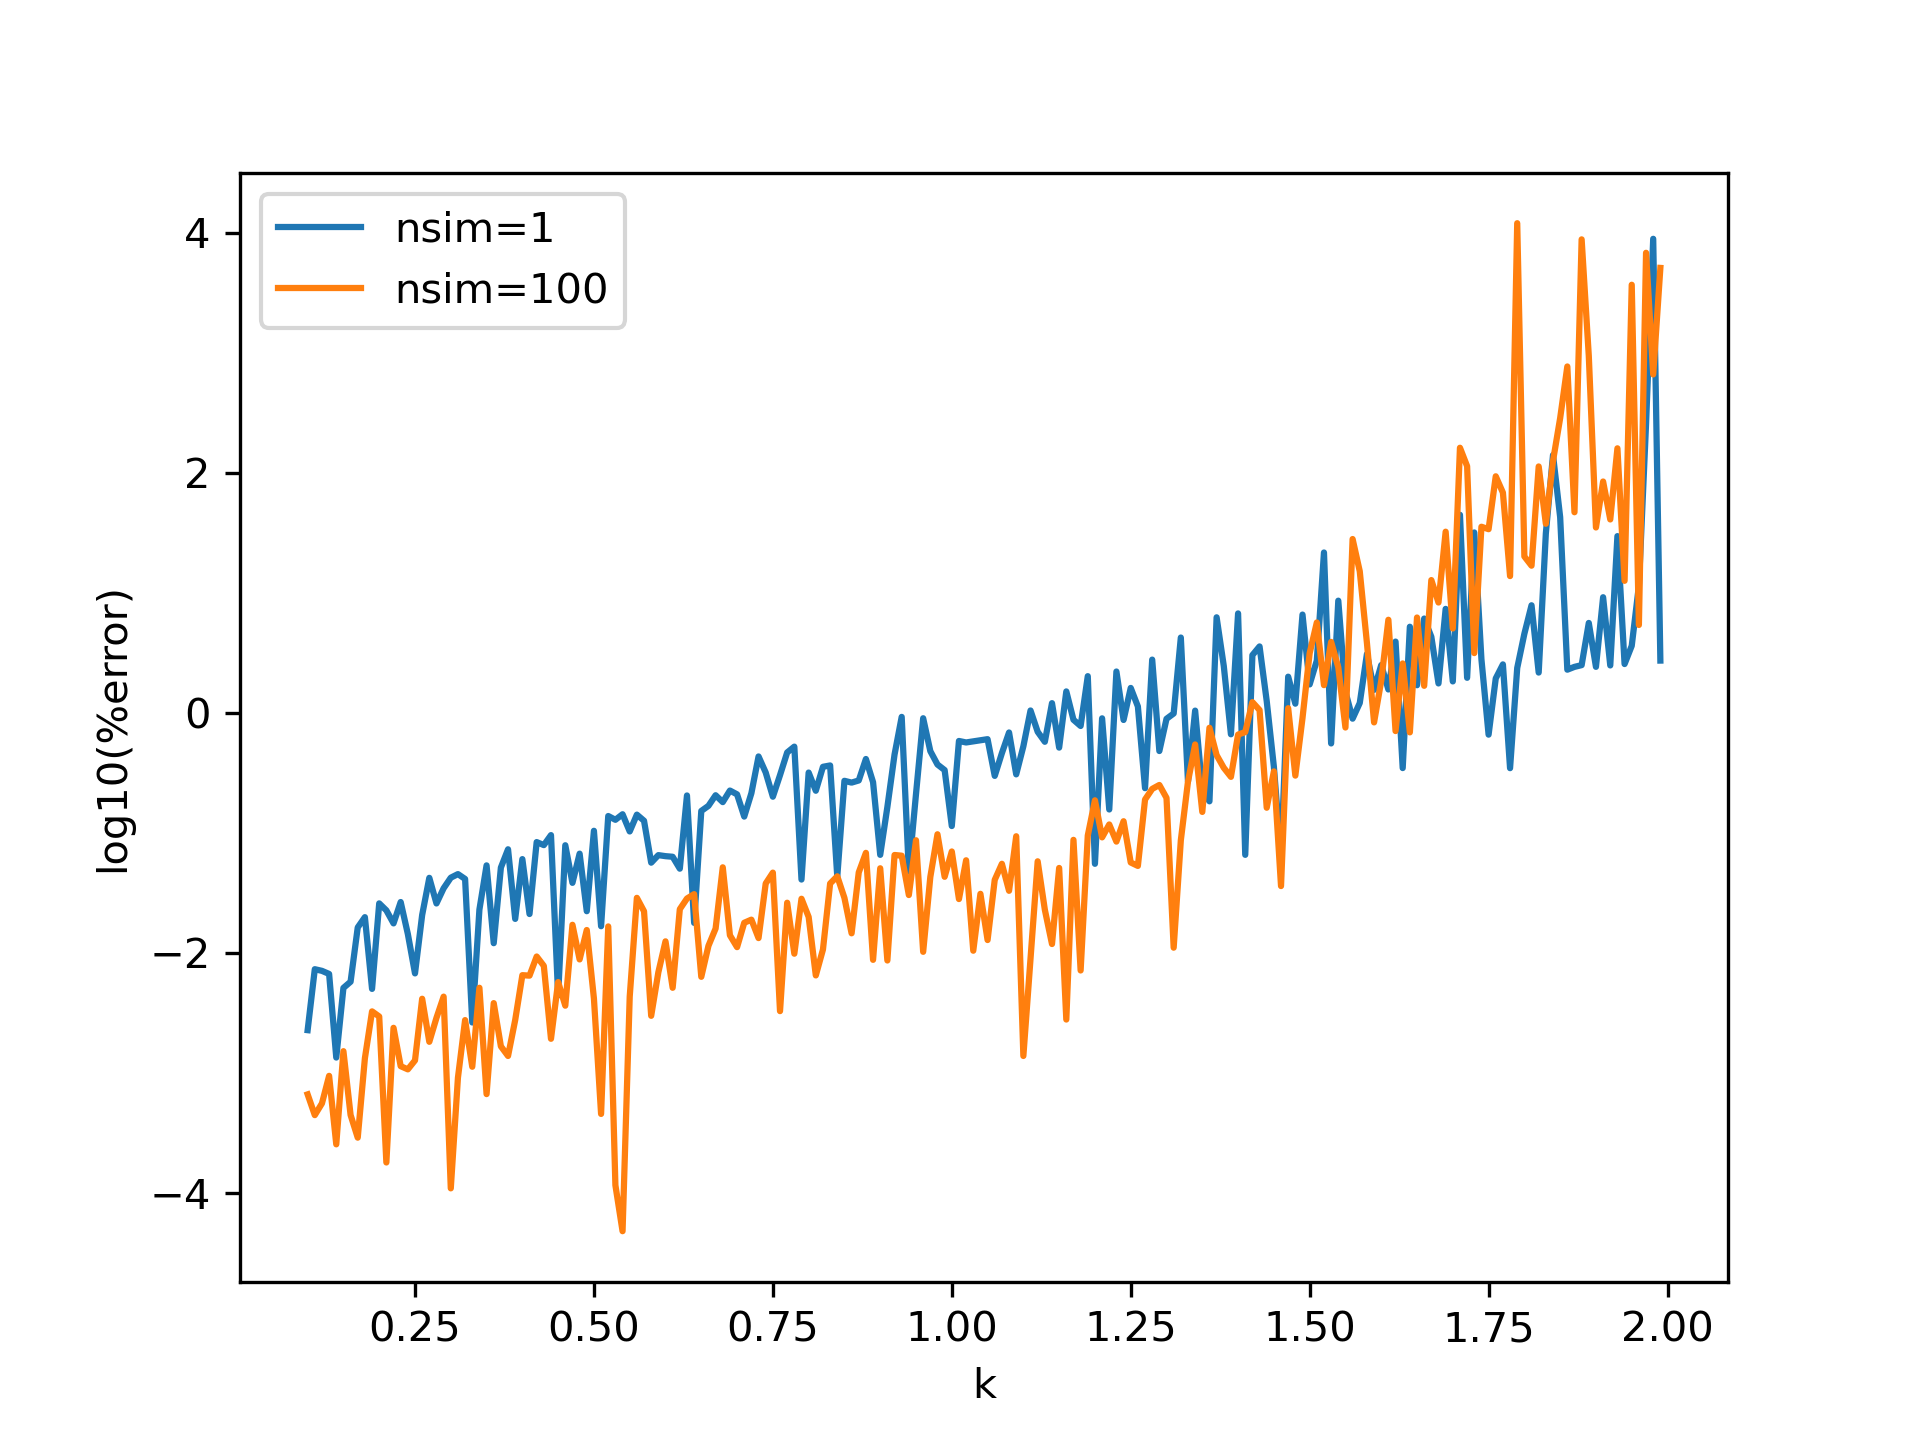
\includegraphics[width=0.8\textwidth]{plots/mainD explosion.png}
    \caption{The logarithmic percentage error of $Y(0)$ for
    (\ref{RRVE:main dirichlet}), with $l=1.2$ and initial conditions
    $y(-k)=e^{-k}$ and $y(k)=e^{k}$, displays an exponential
    increase until approximately $k=1.5$, beyond which additional
    simulations fail to reduce the error, indicating that the variance
    doesn't exist.}
    \label{fig:mainD explosion}
\end{figure}


Here is the Wikipedia article for green functions as a reference:

Green's function

Article
Talk

Read
Edit
View history

Tools

From Wikipedia, the free encyclopedia
This article is about the classical approach to Green's functions. For a modern discussion, see fundamental solution.
An animation that shows how Green's functions can be superposed to solve a differential equation subject to an arbitrary source.
If one knows the solution G ( x , x ′ ) {\textstyle G(x,x')} to a differential equation subject to a point source L ^ ( x ) G ( x , x ′ ) = δ ( x − x ′ ) {\textstyle {\hat {L}}(x)G(x,x')=\delta (x-x')} and the differential operator L ^ ( x ) {\textstyle {\hat {L}}(x)} is linear, then one can superpose them to build the solution u ( x ) = ∫ f ( x ′ ) G ( x , x ′ ) d x ′ {\textstyle u(x)=\int f(x')G(x,x')\,dx'} for a general source L ^ ( x ) u ( x ) = f ( x ) {\textstyle {\hat {L}}(x)u(x)=f(x)}.

In mathematics, a Green's function is the impulse response of an inhomogeneous linear differential operator defined on a domain with specified initial conditions or boundary conditions.

This means that if L {\displaystyle \operatorname {L} } is the linear differential operator, then

the Green's function G G is the solution of the equation L ⁡ G = δ {\displaystyle \operatorname {L} G=\delta }, where δ \delta is Dirac's delta function;
the solution of the initial-value problem L ⁡ y = f {\displaystyle \operatorname {L} y=f} is the convolution ( G ∗ f {\displaystyle G\ast f}).

Through the superposition principle, given a linear ordinary differential equation (ODE), L ⁡ y = f {\displaystyle \operatorname {L} y=f}, one can first solve L ⁡ G = δ s {\displaystyle \operatorname {L} G=\delta _{s}}, for each s, and realizing that, since the source is a sum of delta functions, the solution is a sum of Green's functions as well, by linearity of L.

Green's functions are named after the British mathematician George Green, who first developed the concept in the 1820s. In the modern study of linear partial differential equations, Green's functions are studied largely from the point of view of fundamental solutions instead.

Under many-body theory, the term is also used in physics, specifically in quantum field theory, aerodynamics, aeroacoustics, electrodynamics, seismology and statistical field theory, to refer to various types of correlation functions, even those that do not fit the mathematical definition. In quantum field theory, Green's functions take the roles of propagators.
Definition and uses

A Green's function, G(x,s), of a linear differential operator L = L ⁡ ( x ) {\displaystyle \operatorname {L} =\operatorname {L} (x)} acting on distributions over a subset of the Euclidean space R n \mathbb {R} ^{n}, at a point s, is any solution of
L G ( x , s ) = δ ( s − x ) ,
{\displaystyle \operatorname {L} \,G(x,s)=\delta (s-x)\,,}
(1)
where δ is the Dirac delta function. This property of a Green's function can be exploited to solve differential equations of the form
L u ( x ) = f ( x )   .
    {\displaystyle \operatorname {L} \,u(x)=f(x)~.}
(2)
If the kernel of L is non-trivial, then the Green's function is not unique. However, in practice, some combination of symmetry, boundary conditions and/or other externally imposed criteria will give a unique Green's function. Green's functions may be categorized, by the type of boundary conditions satisfied, by a Green's function number. Also, Green's functions in general are distributions, not necessarily functions of a real variable.
Green's functions are also useful tools in solving wave equations and diffusion equations. In quantum mechanics, Green's function of the Hamiltonian is a key concept with important links to the concept of density of states.
The Green's function as used in physics is usually defined with the opposite sign, instead. That is,
L G ( x , s ) = δ ( x − s )   .
    {\displaystyle \operatorname {L} \,G(x,s)=\delta (x-s)~.}
This definition does not significantly change any of the properties of Green's function due to the evenness of the Dirac delta function.
If the operator is translation invariant, that is, when L {\displaystyle \operatorname {L} } has constant coefficients with respect to x, then the Green's function can be taken to be a convolution kernel, that is,
G ( x , s ) = G ( x − s )   .
    {\displaystyle G(x,s)=G(x-s)~.}
In this case, Green's function is the same as the impulse response of linear time-invariant system theory.
Motivation
See also: Spectral theory
Loosely speaking, if such a function G can be found for the operator L {\displaystyle \operatorname {L} }, then, if we multiply the equation (1) for the Green's function by f(s), and then integrate with respect to s, we obtain,
∫ L G ( x , s ) f ( s ) d s = ∫ δ ( x − s ) f ( s ) d s = f ( x )   .
    {\displaystyle \int \operatorname {L} \,G(x,s)\,f(s)\,ds=\int \delta (x-s)\,f(s)\,ds=f(x)~.}

Because the operator L = L ⁡ ( x ) {\displaystyle \operatorname {L} =\operatorname {L} (x)} is linear and acts only on the variable x (and not on the variable of integration s), one may take the operator L {\displaystyle \operatorname {L} } outside of the integration, yielding
L ( ∫ G ( x , s ) f ( s ) d s ) = f ( x )   .
    {\displaystyle \operatorname {L} \,\left(\int G(x,s)\,f(s)\,ds\right)=f(x)~.}
This means that
u ( x ) = ∫ G ( x , s ) f ( s ) d s
    {\displaystyle u(x)=\int G(x,s)\,f(s)\,ds}













(3)

is a solution to the equation L ⁡ u ( x ) = f ( x )   . {\displaystyle \operatorname {L} u(x)=f(x)~.}

Thus, one may obtain the function u(x) through knowledge of the Green's function in equation (1) and the source term on the right-hand side in equation (2). This process relies upon the linearity of the operator L {\displaystyle \operatorname {L} }.

In other words, the solution of equation (2), u(x), can be determined by the integration given in equation (3). Although f(x) is known, this integration cannot be performed unless G is also known. The problem now lies in finding the Green's function G that satisfies equation (1). For this reason, the Green's function is also sometimes called the fundamental solution associated to the operator L {\displaystyle \operatorname {L} }.

Not every operator L {\displaystyle \operatorname {L} } admits a Green's function. A Green's function can also be thought of as a right inverse of L {\displaystyle \operatorname {L} }. Aside from the difficulties of finding a Green's function for a particular operator, the integral in equation (3) may be quite difficult to evaluate. However the method gives a theoretically exact result.

This can be thought of as an expansion of f according to a Dirac delta function basis (projecting f over δ ( x − s ) {\displaystyle \delta (x-s)}; and a superposition of the solution on each projection. Such an integral equation is known as a Fredholm integral equation, the study of which constitutes Fredholm theory.
See also: Volterra integral equation